% Describe the test setup to verify that your problems from 1.3 have been solved.
% This can be done in different ways depending on focus of your problems.
% Some problems may purely objective, such as "improve the performance of X compared to Y".
% These are easy to evaluate since you simply need to compare the performance, and perhaps compare against a few more technologies that you have listed in Section 2 (related work).
% In other cases the problems may be very subjective, such as "Create a mobile app that can be used while driving, and which shows the most fuel efficient time to change gear".
% This problem will require a user-study in which several persons drive without the application, you calculate the fuel consumption, then they drive with the application and then you calculate the fuel consumption again.
% Then you collect the objective measurements (fuel consumption comparisons) and the subjective opinions from the users about whether the application was unobtrusive, usable, etc. (typically via a questionnaire).

% Move to above section

The testing and comparing of the three diffrent debugger is done manually on some example code, see the git repository \cite{example-code} for the example code.
The example code was many times modified to test how well the three debugger handled the different situations.
This was repeated until one of the debuggers gave an unexpected result.
There were two of these cases found when the code was compiled with optimiation 2.
To keep it fair in these cases a software breakpoint was added to the code.
This ensures that all the three debuggers stops on the same machine code instuction.
The reason being that the debug result can be correct but still different from the other debugger, thus making it seem like one is worse then the other.


\subsubsection{Evalutaion of \emph{Rust} enums}
The \emph{GDB} debugger gave a wrong answer when debugging the value of a enum named \emph{test\_enum3}, the value that \emph{GDB} can be seen in figure \ref{fig:gdbenum}.
The expected value is \emph{TestEnum::Struct(TestStruct { flag: true, num: 123 })} which is not the same as what \emph{GDB} gave.


\begin{figure}[h]
	\centering
	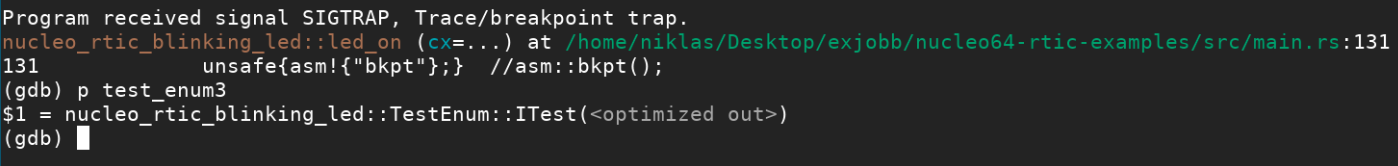
\includegraphics[width=0.9\textwidth]{gdb10.1-opt2-enum-edited.png}
	\caption{\emph{GDB} debugging result from evaluating variable \emph{test\_enum3} when stopped at the software brekpoint in the example code.}
	\label{fig:gdbenum}
\end{figure}


Doing the same using \gls{erd} also gives an unexpected value, the result can be seen in  figure \ref{fig:mydebuggerenum}.
The printing look a bit diffrent but the result from the \gls{erd} debugger tells the user that the enum \emph{test\_enum3} is a enum of type \emph{TestEnum} where the acatual variant has been optimized out.
While \emph{GDB} also tells that \emph{test\_enum3} is of type \emph{TestEnum}, but it also shows thate the enum variant is \emph{ITest}.
As can be seen \emph{GDB} gives the wrong answere because it says that \emph{test\_enum3} is the enum variant \emph{TestEnum::ITest} which is wrong.
While the \gls{erd} debugger shows that the value has been optimized out which is a more correct in this case.


\begin{figure}[h]
	\centering
	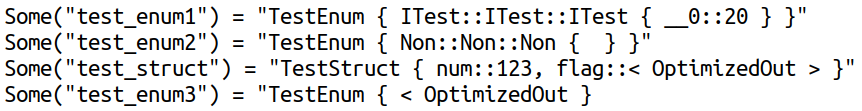
\includegraphics[width=0.9\textwidth]{my-debugger-opt2-enum-edited.png}
	\caption{Debugger presented in this thesis debugging result from evaluating some enum variables when stopped at the software brekpoint in the example code.}
	\label{fig:mydebuggerenum}
\end{figure}


Doing the same using \emph{LLDB} give almost the same result as \gls{erd}, that result can be seen in figure \ref{fig:lldbenum}.
\emph{LLDB} dose not show that the variant of the enum has been optimized out which makes the reason why it is not printed ambigius.


\begin{figure}[h]
	\centering
	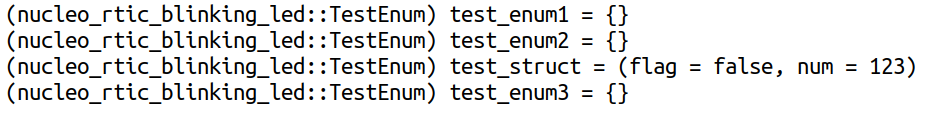
\includegraphics[width=0.9\textwidth]{lldb11.0-opt2-enum-edited.png}
	\caption{\emph{LLDB} debugging result from evaluating some enum variables when stopped at the software brekpoint in the example code.}
	\label{fig:lldbenum}
\end{figure}


Now when inspecting what is stored in the \gls{DWARF} format is shows that the variant of the enum is optimized out but not the two other values that make up the value stored in the variant.
The fact that the value that indicate with variant is optimized out makes it impossible for any debugger to evalute the value stored in the enum.
This is because the encoding of the bytes is unknown and because the number of bytes to read from the stack is unknown.


Looking back at figure \ref{fig:lldbenum} there are three other enums there where two of them dose not have a value as well, they are named \emph{test\_enum1} and \emph{test\_enum2}.
Those two enums should have a value but for some reason \emph{LLDB} is not able to evaluate them, but looking at figure \ref{fig:mydebuggerenum} shows the values they should have.
Also looking at figure \ref{fig:gdbenum} shows the same result as in figure \ref{fig:mydebuggerenum} thus both \emph{GDB} and \gls{erd} is able to evaluate the correct value.
Going back again to figure \ref{fig:lldbenum} which shows that the value of the attribute \emph{flag} is equal to \emph{false}, but looking at figure \ref{fig:gdbenum} and \ref{fig:lldbenum} shows that the value of \emph{flag} is equal to \emph{true}.
The correct value when looking at the original source code is that the attribute \emph{flag} should be equal to \emph{true}, thus meaning that the result from \emph{LLDB} is incorrect.



\subsubsection{Displaying Optimized Out varaibles}
Another problem found is with values that are temporarly not present in any register or the stack which means that it is temporarly optimized out or out of range.
An example of this is the value of the variable \emph{test\_u16} which is a unsinged $16$ bit integer that is temporarly optimized out when stoped at the software breakpoint in the example.
When evaluating this value \emph{GDB} prints that the value is optimized out which can be seen in figure \ref{fig:gdboutofrange}, this is the same output it gives for a value that is totaly optmized out(example of this is the value of \emph{test\_struct} shown in figure \ref{fig:gdbenum}).


\begin{figure}[h]
	\centering
	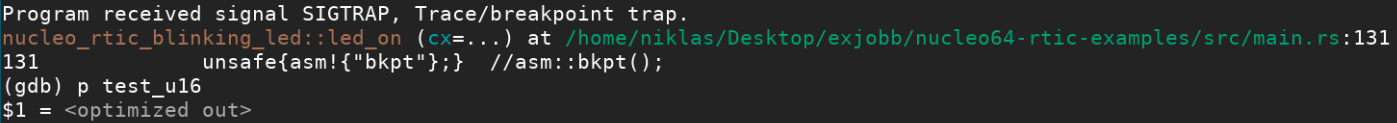
\includegraphics[width=0.4\textwidth]{gdb10.1-opt2-outofrange-edited.png}
	\caption{\emph{GDB} debugging result from evaluating variable \emph{test\_u16} when stopped at the software brekpoint in the example code.}
    	\label{fig:gdboutofrange}
\end{figure}


Doing this with \emph{LLDB} gives the result  \emph{< variable is not available >} which can be seen in figure \ref{fig:lldboutofrange}.


\begin{figure}[h]
	\centering
	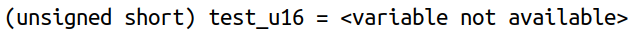
\includegraphics[width=0.9\textwidth]{lldb11.0-opt2-outofrange-edited.png}
	\caption{\emph{LLDB} debugging result from evaluating variable \emph{test\_u16} when stopped at the software brekpoint in the example code.}
	\label{fig:lldboutofrange}
\end{figure}


Lasty compring this to the output of \gls{erd}, which give the value \emph{<OutOfRange>}(see figure \ref{fig:mydebuggeroutofrange}).
The result from both \emph{LLDB} and \gls{erd} are unique and only happen in these situations thus making it easier for the user to understand that the value is temporary optimized out then the reuslt from \emph{GDB}.
This is because the resutl that \emph{GDB} generates is used in multiple situations thus making it unclear if the variable is totaly optimized out or just that is temprarly optimized out.


\begin{figure}[h]
    \centering
    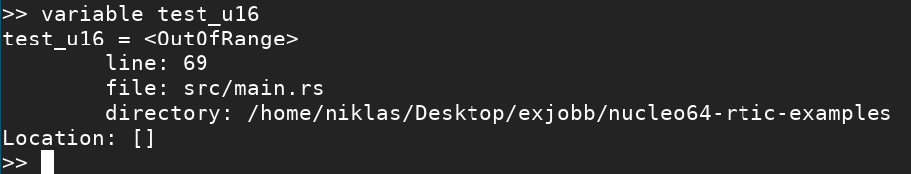
\includegraphics[width=0.9\textwidth]{my-debugger-opt2-outofrange-edited.png}
	\caption{\gls{erd} debugging result from evaluating variable \emph{test\_u16} when stopped at the software brekpoint in the example code.}
    \label{fig:mydebuggeroutofrange}
\end{figure}

